

\begin{exercise}{CIE XYZ Farbmodell}
\label{ex-de-mt-cie}
\begin{itemize}
  \item Erkl�ren sie das CIE XYZ Farbmodell und die wichtigsten ableitbaren Punkte im CIE-XYZ Diagramm (siehe nachfolgende Abbildung).
   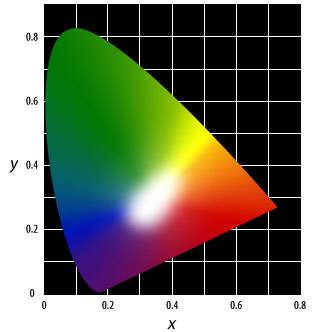
\includegraphics{figure/cie_4}
  \answer{
  \begin{itemize}
  \item Weisspunkt
  \item Black Body Curve - Farbtemperatur
  \item Spektrallinie
  \item Purpurlinie
  \item Gerade WP auf (W Weisspunkt, P Punkt auf der Spektrallinie) zeigt Farben gleicher Farbt�ne
\end{itemize}
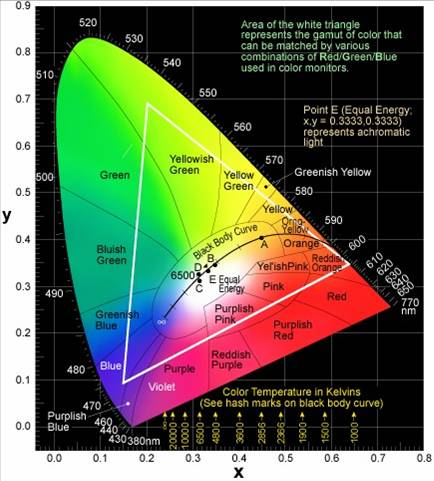
\includegraphics{figure/cie-answer-a}
  }
  \item Welchen Effekt hat ein Wei�abgleich im Diagramm?
  \answer{Er verschiebt den Weisspunkt entlang der Black Body Curve}
  \item Erkl�ren sie den Begriff Gamut und wie der RGB Gamut im CIE-XYZ Farbmodell abgebildet wird.
  \answer{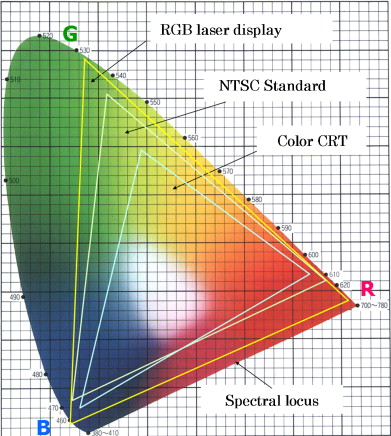
\includegraphics{figure/cie-answer-c-d}}
  \item Nehmen sie zwei RGB Quellen mit unterschiedlichem Farbbereich und unterschiedlicher Farbtemperatur an. Erkl�ren sie damit den Effekt der unterschiedlichen Farbtemperatur auf die dargestellten Farben.
  \answer{Wenn der WP verschoben ist, �ndert sich auch die Farbtonlinie und wird in der N�he von Wei� entsprechend bl�ulicher oder gelber (in Abh�ngigkeit von der Temperatur) } 
\end{itemize}

\end{exercise}

